\documentclass{standalone}
\usepackage{pgfplots}
\pgfplotsset{compat=newest}

\begin{document}
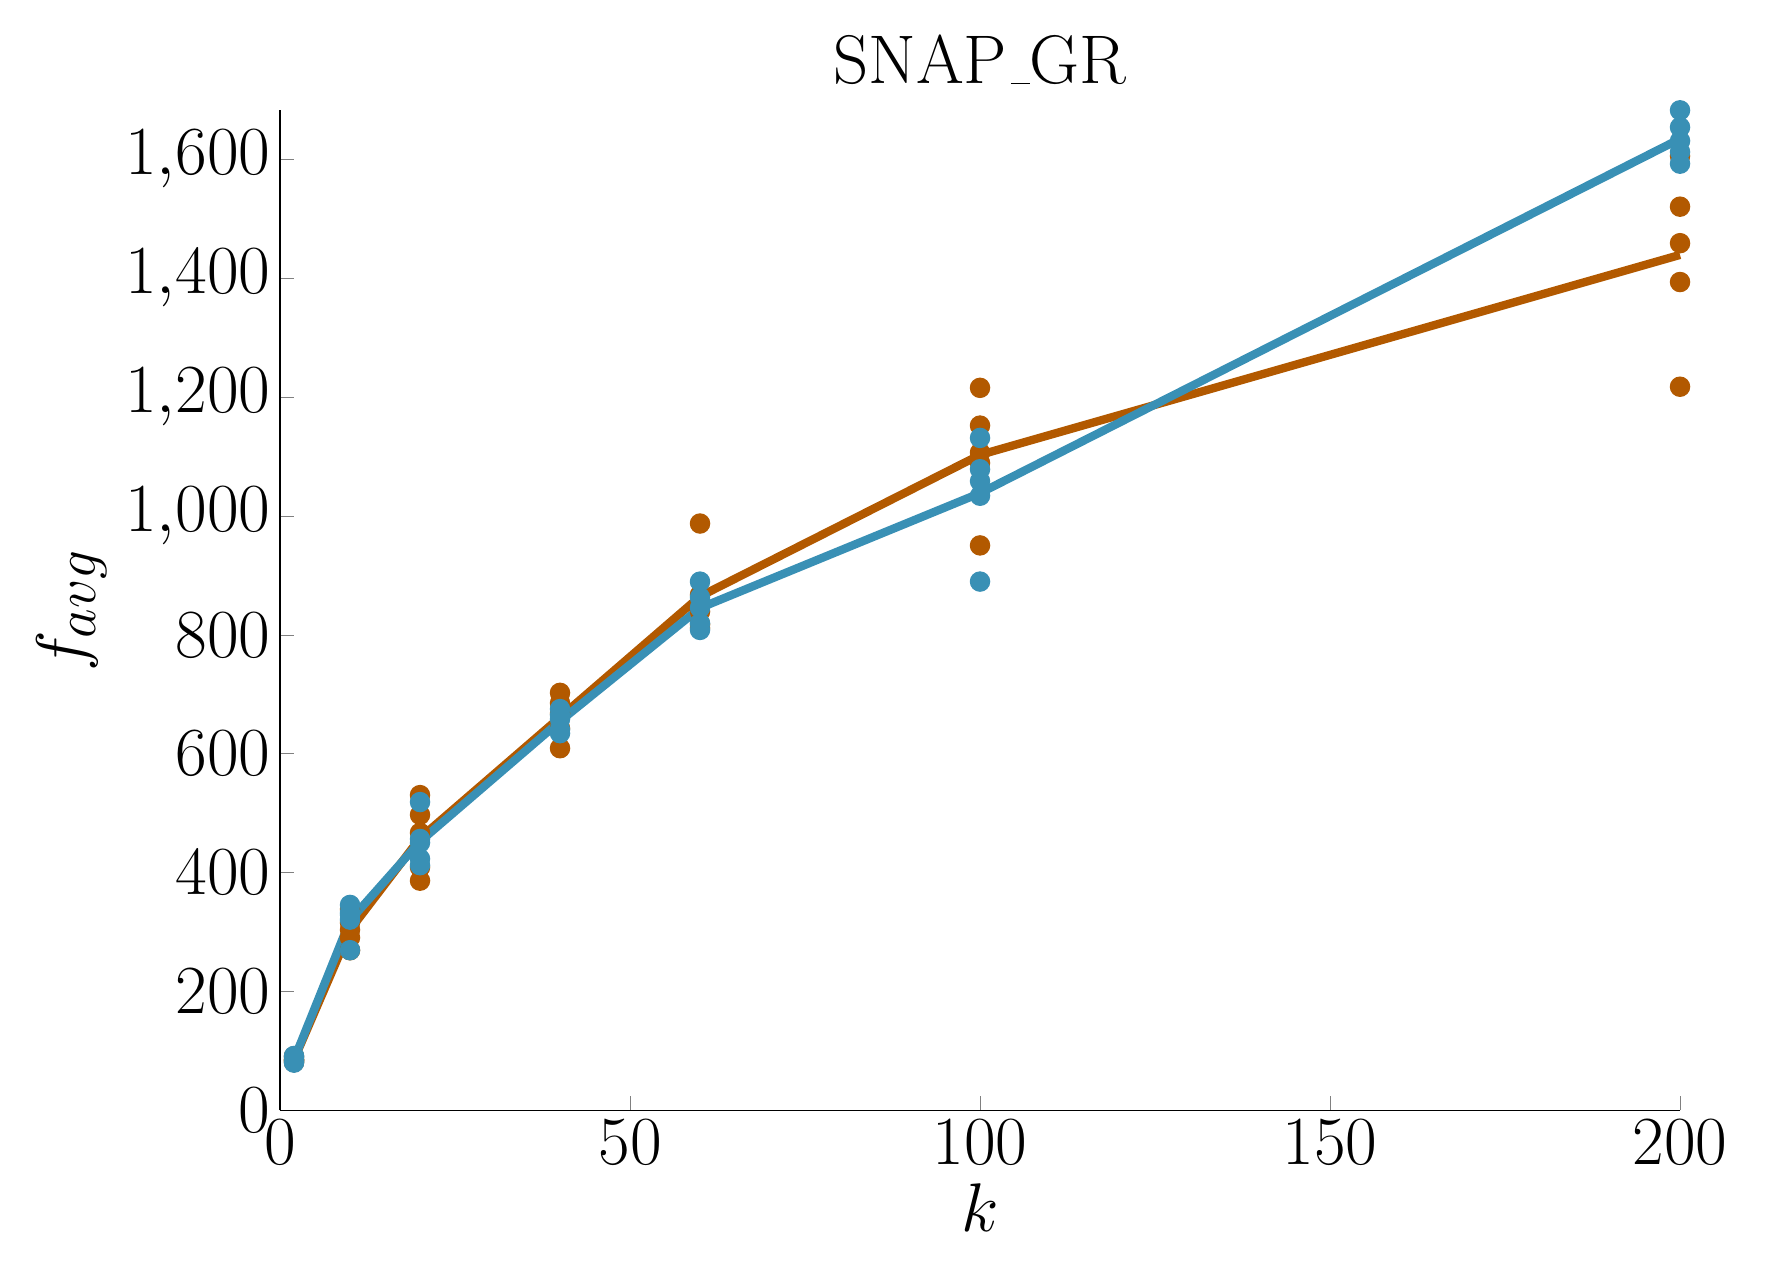
\begin{tikzpicture}

\begin{axis}[%
title style={font=\Huge},
title=SNAP\_GR,
tick label style={font=\Huge},
label style={font=\Huge},
legend style={font=\Huge},
view={0}{90},
max space between ticks=50pt,
width=7in,
height=5in,
scale only axis,
xmin=0, xmax=200,
xtick={0, 50, 100, 150, 200},
xlabel={$k$},
ymin=0, ymax=1682.5,
%ytick={0, 200, 400, 600, 800, 1000},
ylabel={$f_{avg}$},
major tick length=5pt,
axis lines*=left,
legend cell align=left,
clip=false]

\addplot [
only marks,
mark=*,
mark size=3.5pt,
color=orange!70!black,
%solid,
%line width=2pt,
]
coordinates{
(2,80.9)(2,83.85)(2,84.85)(2,85.05)(2,90.75)(10,269.3)(10,290.6)(10,303.65)(10,315.8)(10,338.1)(20,386.35)(20,408.8)(20,466.85)(20,497.15)(20,530.35)(40,609.2)(40,642.65)(40,667.55)(40,685.05)(40,702.4)(60,811.55)(60,817.45)(60,839.3)(60,867.5)(60,987.25)(100,950.45)(100,1089.2)(100,1106.75)(100,1152.05)(100,1215.55)(200,1217.45)(200,1393.6)(200,1458.95)(200,1520.35)(200,1605.7)
};

\addplot [
only marks,
mark=*,
mark size=3.5pt,
color=cyan!70!black,
%solid,
%line width=2pt,
]
coordinates{
(2,80.2)(2,81.7)(2,84.55)(2,89.25)(2,91.45)(10,269.45)(10,320.8)(10,329.25)(10,332.75)(10,345.55)(20,412.4)(20,423.0)(20,450.3)(20,456.5)(20,518.65)(40,634.5)(40,640.55)(40,658.3)(40,664.65)(40,675.1)(60,808.25)(60,819.45)(60,845.55)(60,863.0)(60,889.5)(100,889.6)(100,1034.0)(100,1058.6)(100,1078.65)(100,1131.3)(200,1592.7)(200,1612.5)(200,1631.05)(200,1654.05)(200,1682.5)
};

\addplot [
color=orange!70!black,
solid,
line width=3pt
]
coordinates{
(2,85.08)(10,303.49)(20,457.9)(40,661.37)(60,864.61)(100,1102.8)(200,1439.21)
};

\addplot [
color=cyan!70!black,
solid,
line width=3pt
]
coordinates{
(2,85.43)(10,319.56)(20,452.17)(40,654.62)(60,845.15)(100,1038.43)(200,1634.56)
};


\end{axis}
\end{tikzpicture}
\end{document}
